\section{Volumetric displays}

Volumetric displays \cite{1492264} are a promising technology that offers a captivating three-dimensional viewing experience. By emitting light for each voxel, or volume element, in a 3D space, these displays transcend the limitations of traditional 2D planes, providing a truly immersive 3D effect. This innovative approach enables the accurate representation of virtual 3D objects, including focal depth, motion parallax, and vergence, which refers to the rotation of a viewer's eye to fixate on the same point they are focusing on. Moreover, volumetric displays allow multiple users to view the same display from different angles, providing unique perspectives of the same object.

\subsection{Swept Volume Displays}
Swept volume displays represent one category of volumetric displays. They employ a moving 2D display to create a 3D image. This is achieved by moving the 2D display through a 3D space and emitting light from the display at each point. Common techniques for achieving this includes using a rotating mirror \cite{10.1117/12.480930}, emitting screen typically an LED \cite{Gately:11}, or transparent projector screen \cite{keane_volumetric_2016}. There currently exist commercial products that implement this as can be seen in Fig~\ref{fig:swept-volume-displays}.

\begin{figureBox}[label={fig:swept-volume-displays}]{Two different types of swept volume display}
  \begin{minipage}[t]{0.48\textwidth}
    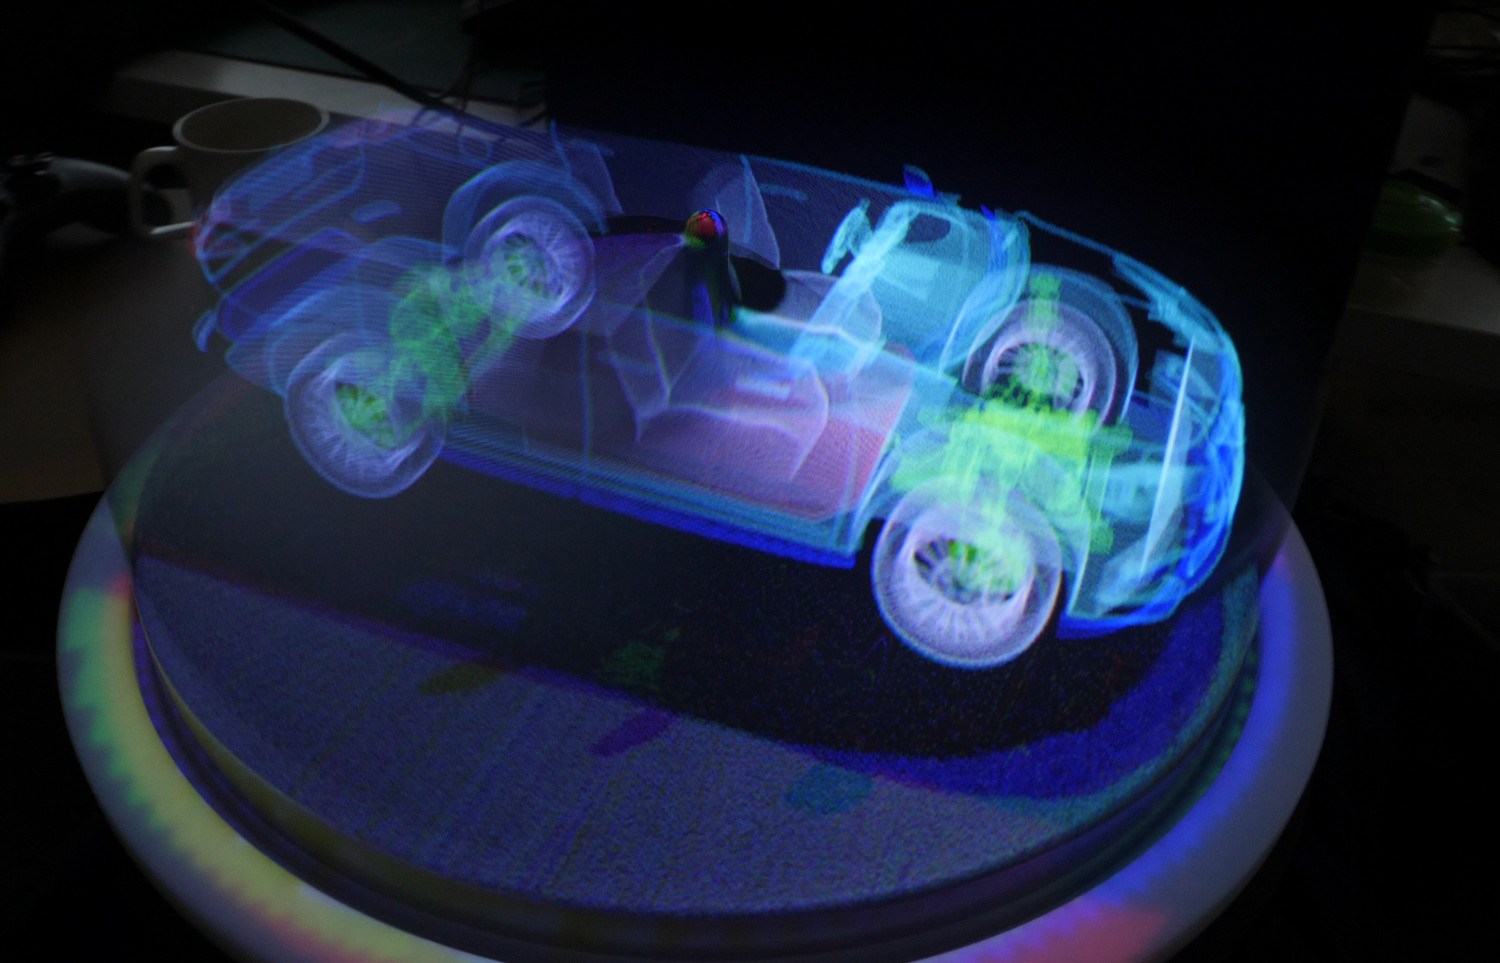
\includegraphics[width=\textwidth]{./background/figures/3d/voxon.jpg}
    \small {a) The VXR4612 3D Volumetric Display, a projector based persistence of vision display produced by Voxon Photonics. \tocite}
  \end{minipage}\hfill
  \begin{minipage}[t]{0.48\textwidth}
    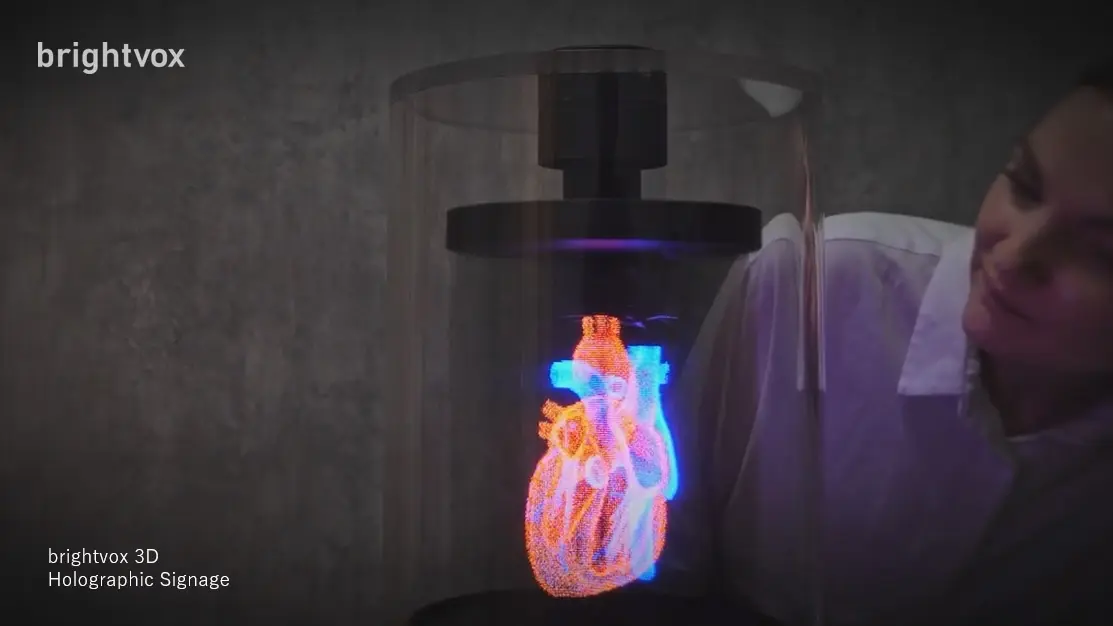
\includegraphics[width=\textwidth]{./background/figures/3d/brightvox.png}
    \small {b) A Volumetric Display / Holographic Signage, a LED based persistence of vision display produced by Brightvox Inc. \tocite}
  \end{minipage}
\end{figureBox}

\subsection{Static Volume Displays}
Static volume displays are another category of volumetric displays. They employ a static 3D display to create a 3D image. This is achieved by emitting light from the display at each point in a 3D space. Techniques for achieving this range from using a 3D array of LEDs \cite{10.1145/2341931.2341937}, lasers and phosphorus gas \cite{https://doi.org/10.1002/anie.202003160}, or a transparent laser induced damaged medium that can be projected into \cite{10.1145/1179849.1179982}.

\subsection{Trapped Particle displays}
{\textcolor{red}{TODO}}

\subsection{Photon displays}
{\textcolor{red}{TODO}}

\subsection{Issues}

Expensive: Swept volume displays require extremely high refresh rate projectors, which are expensive and difficult to manufacture or transparent LED screens which are only recently becoming widely available. For example the Voxon VX1 one of the few if only commercial available volumetric displays costs \$11,700 USD \cite{noauthor_products_nodate}. \\

High bandwidth requirements: To render objects in real time at 2D display equivalent resolutions while taking a raw voxel stream (as apposed to calculating voxels on hardware from primitive shapes) has an extremely high bandwidth requirement. \texttt{60fps} on a $4096 \times 2160 \times 1080$ voxel display with \texttt{24 bit} color requires a bandwidth of $1.37 \times 10^3$ bits per second/13.7 terabits per second. To achieve that currently would require about 170 state-of-the-art Ultra High Bit Rate (UHBR) (80 gigabit) DisplayPort cables simultaneously. It was predicted in 2021 \cite{LAM2021050011} that a based on the historical trend of display bandwidth that a volumetric 4K screen will become feasible in 2060.

\subsection{Volumetric Screen Simulations}
Because of the high cost and bandwidth requirements of volumetric displays, there has been some research into simulating volumetric displays on traditional 2D displays. One commonly used method is the so called fish tank virtual reality (FTVR) display \cite{10.1145/3290605.3300763} \cite{Zabarauskas2012}